%---------------------导言区---------------------------%
\documentclass[12pt,a4paper,UTF8]{ctexart}
	%10pt:正文字体为12pt,缺省为10pt;各层级字体大小会根据正文字体自动调整
	%a4paper:纸张大小a4;
	%UTF8:中文要求
%\usepackage{syntonly}
%\syntaxonly%加快编译速度
\usepackage{geometry}%用于设置上下左右页边距
	\geometry{left=2.5cm,right=2.5cm,top=3.2cm,bottom=2.8cm}
\usepackage{xeCJK,amsmath,paralist,enumerate,booktabs,multirow,graphicx,float,subfig,setspace,listings,lastpage,hyperref,gensymb}
	%xeCJK:中文字体(如楷体,作者和机构需要用到)的设置
	%amsmath:数学公式
	%paralist,enumerate:自定义项目符号
	%booktabs:三线图,论文常用的表格风格
	%multirow:复杂表格
	%graphicx,float: 插入图片
	%subfig:并排排版图片以及强制图表显示在“这里”[H]
	%setspace:设置行间距等功能
	\setlength{\parindent}{2em}%正文首行缩进两个汉字
	%listings:用于排版各种代码;比如matlab的代码
	%\lstset{language=Matlab}%matlab代码
	%lastpage:获取总页数;
	%hyperref:超链接,和lastpage搭配.
\usepackage{fancyhdr}
	%fancyhdr:一个很强大的宏包,用于自定义设计页面风格并命名以供调用。
	\pagestyle{fancy}
	\rhead{实验二十一~观察光的偏振现象}
	\lhead{普通物理实验\uppercase\expandafter{\romannumeral1}实验报告}
	\cfoot{\thepage}  
		%分别是右页眉、左页眉、右页脚
	\renewcommand{\headrulewidth}{0.4pt}
	\renewcommand{\theenumi}{(\arabic{enumi})}

\setCJKmainfont{FZSSK.TTF}[ItalicFont=FZKTK.TTF, BoldFont=FZHTK.TTF]
%中文字体设置:使用开源字体方正书宋,方正楷体和方正黑体



%%%%%%%%%%%%%%%%%%%%%%%%%%%%%%%%%%%%%%%%%%%%%%%%%%%%%%%%%%
%%%%%%%%%%%%%%%%%%%%%%%%%正文开始%%%%%%%%%%%%%%%%%%%%%%%%%%
%%%%%%%%%%%%%%%%%%%%%%%%%%%%%%%%%%%%%%%%%%%%%%%%%%%%%%%%%%

\begin{document}

%%begin-------------------标题与信息-----------------------%%

%%标题
\begin{center}
\LARGE\textbf{实验二十一~观察光的偏振现象}
\end{center}

%%信息
\begin{doublespacing}
	%doublespacing:手动两倍行距
	\centering
	\begin{tabular}{lr}
	 & \\
	{\CJKfontspec{STKAITI.TTF} 实验人:钟易轩(2000012706)} & {\CJKfontspec{STKAITI.TTF}指导教师:曲波}\\
	{\CJKfontspec{STKAITI.TTF} 实验时间:2021年10月22日~星期五~下午} &{\CJKfontspec{STKAITI.TTF} 实验地点:物理楼南楼~341}
	\end{tabular}
\end{doublespacing}

%%end-------------------标题与信息-----------------------%%


\subsection*{【实验目的】}
	\begin{enumerate}[(1)]
		\item 验证布儒斯特定律
		\item 观察双折射现象
		\item 产生和观察光的偏振状态
		\item 了解产生与检验偏振光的元件和仪器
		\item 掌握产生与检验偏振光的条件和方法
	\end{enumerate}

\subsection*{【仪器用具】}

	\paragraph{偏振光镜、偏振片、方解石块、1/2波片、1/4波片,激光器,钠光灯、玻璃片堆}

\subsection*{【实验原理】}

	\subsubsection*{1.光的偏振态}
%% 自然换段:\par
	我们知道的常见的光大体上分为五种偏振态,即线偏振光、圆偏振光、椭圆偏振光、自然光和部分偏振光。其中的线偏振光和圆偏振光可看作椭圆偏振光的特例。由于在产生感光作用和生理作用的是光波的电矢量E,因此在进行偏振讨论时只考虑电矢量E。
	
	\subsubsection*{2.布儒斯特角}

	在特定入射角即布儒斯特角$\theta$入射时,不管入射光的偏振态怎样,反射光都会变成线偏振光。\par
	例:如果光以空气入射到折射率为n的玻璃平面上,则$\theta$=$\arctan$~n。如果自然光以$\theta$入射到玻璃片堆上,则经多次反射,最后从玻璃片堆透射出来的光一般是部分偏振光。如果玻璃片数目较大,则透射光近似为线偏振光。

	\subsubsection*{3.偏振片}

	实验发现有些晶体对不同偏振状态的光有选择吸收的性质。当光的电矢量与晶体的光轴平行时,光被晶体吸收较少,而电矢量与光轴垂直时,光被吸收较多。这种性质叫做晶体的二向色性,利用它便可以制作偏振片。例如,常见的偏振片是在拉伸了的赛珞基片上蒸镀一层硫酸碘奎宁小晶粒,利用晶片的应力使晶粒的光轴定向排列,构成面积较大的偏振片。\par
	自然光经过偏振片其透射光基本上为线偏振光。

	\subsubsection*{4.波晶片}

	一束光在晶体里传播使被分成两束折射程度不同的光,这种现象叫做光的双折射现象。两束光线中,一束符合折射定律,叫做寻常光(o光),而另一束光线不符合折射定律,叫做非寻常光(e光)。晶体中还有一个特殊方向,当光线沿着该方向传播时,不会分成o光和e光,这个方向叫做晶体的光轴。只有一个光轴方向的晶体叫做单轴晶体,具有两个光轴方向的晶体称作双轴晶体。\par
	利用单轴晶体的双折射,产生的寻常光(o光)和非寻常光(e光)都是线偏振光。前者的电矢量E垂直于o光的主平面(晶体内部某条光线与光轴构成的平面),后者的E平行于e光的主平面。\par
	波晶片是从单轴晶体中切割下来的平面平行板,其表面平行于光轴,它也叫做相位延迟板。当一束平行自然光正入射到波晶片上,光在晶体内部分解为o光和e光。但是o光在晶体内的波速为$\upsilon_o$,e光在晶体内的波速为$\upsilon_e$,因此它们的折射率也不一样,则通过波片后的光程也会有所不同。\par
	设晶体的厚度为d,则两束光经过晶片后就有相位差
	\begin{equation}
		\delta=\frac{2\pi}{\lambda}(n_o-n_e)l
	\end{equation}
\par
	$\delta$=2k$\pi$的晶片称为全波片;$\delta$=2k$\pi$+$\pi$的叫做半波片($\lambda$/2片);$\delta$=2k$\pi$的叫做$\lambda$/4片。
\subsection*{【实验内容】}

	\subsubsection*{1.用偏振光镜验证布儒斯特定律}
	\begin{enumerate}[(1)]
			\item 使玻璃片堆A平行于玻璃片P,绕z轴转A,观察A的反射光的强度变化,并简要解释之。
			\item 同(1),但观察透射光的强度变化,并予以解释。
	\end{enumerate}
	\subsubsection*{2.观察双折射现象}
	\begin{enumerate}[(1)]
			\item 以小灯照明铝板上的小孔,孔上放方解石\uppercase\expandafter{\romannumeral1}(负单轴晶体),通过它观察小孔,转动方解石。记录所见现象并加以思考。
			\item 将方解石块\uppercase\expandafter{\romannumeral2}放在小孔上(磨面压小孔),作同样的观察。
			\item 利用一透光方向已知的偏振片,判断寻常光与非寻常光电矢量的振动方向,记录并解释之。
	\end{enumerate}
	\subsubsection*{3.观察线偏振光通过$\lambda$/2片后的现象}
	\begin{enumerate}[(1)]
			\item 了解偏振片P,A的作用,在观察者与光源S之间,放入偏振片P,旋转P,看透射光的强度有无变化。再放上检偏器A,转A,观察光透过A的强度怎样变化。
			\item 使P的透光方向竖直(是否必须竖直?),转A达到消光。在P,A间插入半波片,将半波片转动360\degree,能看到几次消光,试加以解释。
			\item 把半波片任意转动一角度,破坏消光现象,再将A转动360\degree,又能看到几次消光?
			\item 仍使P的透光方向竖直,P,A正交,插入$\lambda$/2片,转之使消光(此时$\lambda$/2片的e轴或者o轴以及P的透光方向都沿着竖直方向)。以此时P和$\lambda$/2片位置对应角度为$\theta$=0\degree,保持$\lambda$/2片不动,将P转$\theta$=15\degree,破坏消光,再沿与转P相反的方向转A至消光位置,记录A所转过的角度$\theta^{\prime}$。
			\item 继续(4)的实验,依次使$\theta$=30\degree,45\degree,60\degree,75\degree,90\degree($\theta$值是相对P的起始位置而言),转A到消光位置,记录相应的角度$\theta^{\prime}$。
	\end{enumerate}
	从上面实验结果能总结出什么规律?
	\subsubsection*{4.用$\lambda$/4片产生椭圆偏振光}
	\begin{enumerate}[(1)]
			\item 取下半波片,仍使P的透光方向竖直,P与A正交。插入$\lambda$/4片,转之使消光。
			\item 保持$\lambda$/4片不动,将P转$\theta$=15\degree,然后将A转360\degree,观察光强变化。
			\item 继续(2),依次使$\theta$=30\degree,45\degree,60\degree,75\degree,90\degree,每次将A转360\degree,观察光强的变化,根据观察结果画图或用文字说明透过$\lambda$/4片的出射光的偏振状态。
	\end{enumerate}
	\subsubsection*{5.检验椭圆偏振光与部分偏振光}
	根据实验室提供的元件(三块偏振片,两块$\lambda$/4片和一玻璃片堆),自行设计实验方案,产生并检验椭圆偏振光和部分偏振光。

\subsection*{【实验记录及分析】}
	\subsubsection*{1.用偏振光验证布儒斯特定律}
	\begin{enumerate}[(1)]
		\item 反射光在转动的360\degree 里面,出现了两次消光,分别是在90\degree、270\degree 的时候,也出现了两次光强极大值点,分别是0\degree 和180\degree 的时候。原因是激光经过P的反射之后,由于是以布儒斯特角入射,则反射光为线偏振光。当A与P平行时,根据马吕斯公式,光强最大,当A转动90\degree 或270\degree 时,$\cos\theta=0 $,即消光。
		\item 透射光与反射光的变化相反,究其原因是能量守恒定律的影响。
	\end{enumerate}

	\subsubsection*{2.观察双折射现象}
	\begin{enumerate}[(1)]
		\item 可以看见两个光点,在方解石旋转的过程中,一光点动,另一光点不动,动的光点应该是非寻常光,而不动的光点是寻常光。原因是o光遵守折射定律,e光不遵守折射定律。
		\item 在磨面上能看到一不动的光点,说明磨面所在轴便是光轴,因为光沿光轴入射才不会分解。
		\item 在(2)中我们确定了光轴方向,再放上方解石\uppercase\expandafter{\romannumeral1},将已知透振方向的偏振片沿着方解石的光轴摆放,发现只有一个亮点,转动偏振片,发现两个亮点,继续转动到90度左右时,只有一个亮点,证明了o光和e光的电矢量方向垂直。
	\end{enumerate}

	\subsubsection*{3.观察线偏振光通过$\lambda$/2片后的现象}
	\begin{enumerate}[(1)]
			\item 偏振片P作为起偏器,偏振片A作为检偏器;未放置A时,转动P观察到的透射光无变化,因为P产生的线偏振光的光强没变;放上A之后,旋转A会使亮度变化,且会发生消光现象,因为马吕斯公式 $ I_{\theta}=I_{0}\cos^{2}\theta $,在转动A时,A与P的透振方向之间的夹角$\theta$发生了变化,从而光强也发生变化,当$\theta$=90\degree,出现消光现象。
			\item 出现四次消光。因为光的偏振在e-o轴中,假如偏振方向与e轴或o轴平行,那么偏振方向在穿过波晶片后不会发生改变,即以原偏振方向射出,自然会消光,$\lambda$/2片在转动过程中会出现2*2=4次消光现象。
			\item 看到两次消光现象。线偏振光穿过$\lambda$/2片之后的偏振方向已经确定,由于A的透振方向需要与其垂直才能消光,则应有360\degree /180\degree =2次消光现象。
			\item $\theta^{\prime}$=-13\degree 
			\item 如下表所示,在误差范围内,有$\theta$=-$\theta^{\prime}$,且线偏振光经$\lambda$/2片后振动方向转过的角度为2$\theta$。
	\end{enumerate}
	
	\begin{table}[htbp]
	  \centering
	\caption{$\lambda$/2片转动影响偏振态的观察记录}
	    \begin{tabular}{c|c|c}
			\hline
	    	\textbf{$\theta$} & \textbf{$\theta^{\prime}$} & \textbf{线偏振光经$\lambda$/2片后振动方向转动的角度}\\
			\hline
			$0\degree$ & $0\degree$ & $0\degree$ \\
			$15\degree$ & $-13\degree$ & $28\degree$ \\
			$30\degree$ & $-28\degree$ & $58\degree$ \\
			$45\degree$ & $-41\degree$ & $86\degree$ \\
			$60\degree$ & $-59\degree$ & $119\degree$ \\
			$75\degree$ & $-73\degree$ & $148\degree$ \\
			$90\degree$ & $-88\degree$ & $178\degree$ \\
			\hline
	    \end{tabular}
	\end{table}
	\subsubsection*{4.用$\lambda$/4片产生椭圆偏振光}
	\begin{enumerate}[(1)]
		\item 略
		\item 由亮变暗,再由暗变亮,又由亮变暗,最后由暗变亮。(每一个过程所转过的角度为90\degree)
		\item 如表所示(注:每一个小过程皆是90\degree)
	\end{enumerate}
	
	\begin{table}[htbp]
	  \centering
	\caption{$\lambda$/4片转动影响偏振态的观察记录}
	    \begin{tabular}{c|c|c}
			\hline
	    	\textbf{$\theta$} & \textbf{A转动360\degree 观察到的现象} & \textbf{光的偏振状态}\\
			\hline
			$0\degree$ & 先变亮再变暗至消光再变亮再变暗至消光再变亮回原来亮度 & 线偏振 \\
			$15\degree$ & 先变亮再变暗再变亮再变暗  &  椭圆偏振  \\
			$30\degree$ &  先变亮再变较暗再变亮再较暗  &  椭圆偏振  \\
			$45\degree$ &  亮度几乎无变化  &  圆偏振  \\
			$60\degree$ &  先变暗再变亮再变暗再变亮  & 椭圆偏振 \\
			$75\degree$ &  先变暗再变亮再变暗再变亮  &  椭圆偏振  \\
			$90\degree$ &  先变暗至消光再变亮再变暗至消光再变亮  &  线偏振  \\
			\hline
	    \end{tabular}
	\end{table}
	\subsubsection*{5.检验椭圆偏振光与部分偏振光}
	
	\begin{enumerate}[(1)]
\item 检验椭圆偏振光:首先用光源、起偏器、$\lambda$/4片和检偏器构造一个椭圆偏振光,然后调节检偏器使得透射光光强最大时候(即检偏器透振方向是椭圆长轴方向),再插入$\lambda$/4片使得其光轴与椭圆长轴方向平行,此时再转动检偏器,发现消光现象,说明原偏振光是椭圆偏振光。
\begin{figure}[htbp]
		\centering
		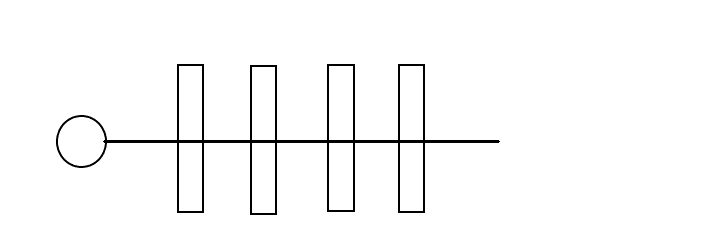
\includegraphics{1.png}
		\caption{检验椭圆偏振光示意图}
	\end{figure}
\item 检验部分偏振光:首先用光源、玻璃片堆构造一个部分偏振光,再用检偏器旋转着去检查,发现只有光的明暗变化,并未消光,则判定出是部分偏振光。
\begin{figure}[htbp]
		\centering
		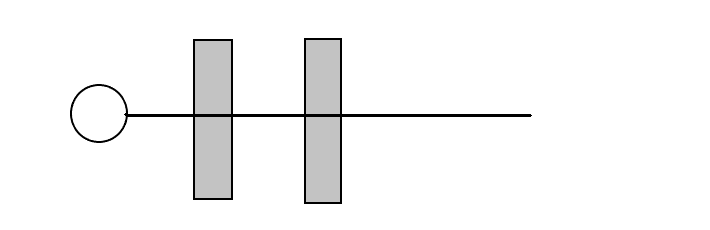
\includegraphics{2.png}
		\caption{检验部分偏振光示意图}
	\end{figure}
	\end{enumerate}

\subsection*{收获与感想}

	
	\begin{enumerate}[(1)]
			\item 在课堂上接触了诸如偏振片、波晶片之类的光学元件,我在学会理论分析的同时也真实感受到了不同于“纸上谈兵”的直面物理现象的体验,也对照相机等装备的偏振片的使用方法也有了更深的体会。
			\item 利用偏振现象,我也更直观地感受到了光的传播,对光的波动性有了更深的理解与认识。
	\end{enumerate}

\subsection*{参考文献}

《新编基础物理实验》(第二版)\qquad 吕斯骅\quad 段家怟\quad 张朝晖\quad 主编
	


\newpage %换页




\end{document}
